\section{Tabular Prior-Data Fitted Network Transformations and Dataset Construction}
\label{sec:transformations}

\subsection{Purpose and scope}
\label{sec:transforms:scope}

This section describes 2 ways in which the processed Surveillance,
Epidemiology, and End Results (SEER) cohorts were transformed using a Tabular
Prior-Data Fitted Network (TabPFN) \citep{Hollmann2025}. The first transformation creates a numerical
embedding for every real patient. An embedding replaces the original clinical
variables with a vector of numbers intended to summarise the information that
TabPFN learned from those variables and the task outcome. The second
transformation creates entirely new synthetic records by learning a distribution
over the clinical predictors and outcomes and then sampling from it.

The 2 transformations serve different purposes. Embeddings retain the original
patients and outcomes but change how their clinical information is represented.
Synthetic generation retains the original clinical column structure but creates
new combinations of predictors and outcomes. The resulting datasets are used in
later sections to examine predictive performance and the extent to which the
synthetic records resemble the real cohorts.

Both transformations in this section were created once from the complete
diagnostic or prognostic cohort. This is important for interpretation. They are
suitable for studying the fixed transformed datasets, but they do not provide an
independent evaluation of a transformation learned using training data alone.
The later augmentation experiment therefore generates synthetic records
separately within each training portion and evaluates the resulting models only
on real patients that were not used by the generator.

\begin{figure}[htbp]
\centering
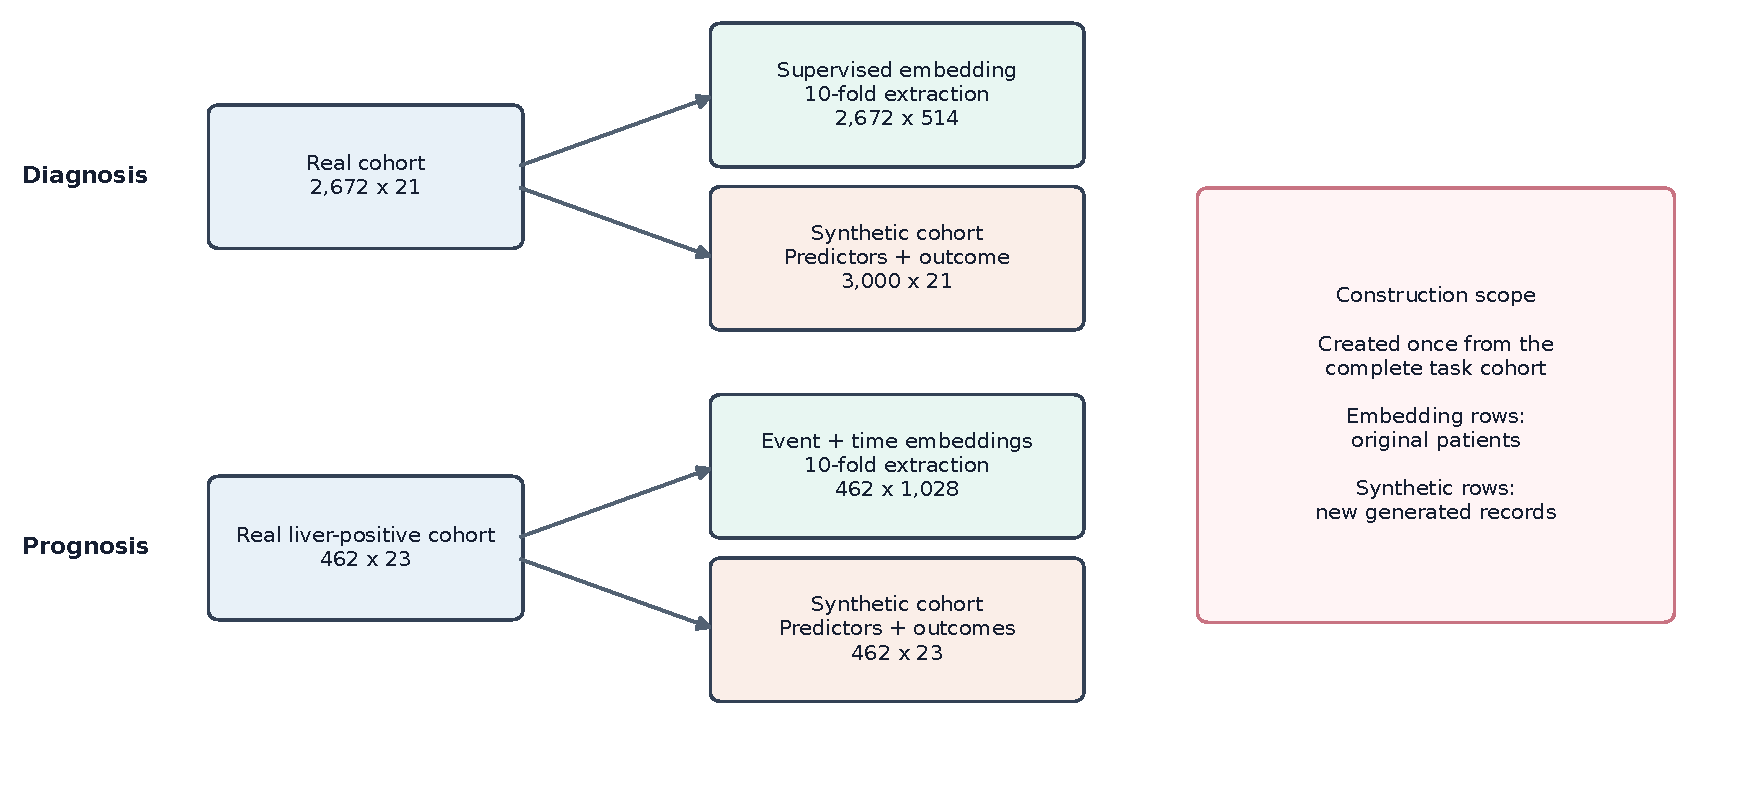
\includegraphics[width=\linewidth]{tabular_transformations/transformation_flow.pdf}
\caption{Transformation routes and resulting dataset dimensions. Embedding rows
represent the original patients and retain their outcomes. Synthetic rows are
newly generated records containing clinical predictors and outcomes. Both
transformations shown here were constructed once from the complete cohort for
the corresponding task.}
\label{fig:transforms:flow}
\end{figure}
\FloatBarrier

\subsection{Input variables and resulting datasets}
\label{sec:transforms:inventory}

Both transformations start from the diagnostic and prognostic cohorts described
in Section~\ref{sec:data}. Each task contains 19 clinical predictor columns. This
input is wider than the 17 clinical descriptor families considered during the
reference-model variable-selection stage because 2 clinical concepts appear in
2 forms. Nodal stage is represented both as the American Joint Committee on
Cancer N category and as a binary indicator of nodal involvement. Tumour size is
represented both as an exact measurement in millimetres and as a grouped
category. Comparisons with the reference models therefore reflect both a new
numerical representation and a broader input specification.

Patient identifiers were retained only to match transformed rows to their
corresponding patients and were never used as model inputs. For diagnosis, liver
metastasis at diagnosis is the outcome. For prognosis, death status and observed
follow-up time in months form the outcome. Liver-metastasis status is retained in
the prognostic dataset for consistency, but it is not used as a predictor because
all 462 patients in that cohort have liver metastasis.

\begin{table}[htbp]
\centering\footnotesize
\caption{Inputs and resulting data for each transformation. Predictor counts
exclude patient identifiers and outcomes.}
\label{tab:transforms:schema}
\begin{tabularx}{\linewidth}{@{}p{0.16\linewidth}p{0.12\linewidth}p{0.23\linewidth}p{0.22\linewidth}Y@{}}
\toprule
Route & Task & Input to transformation & Outcome information & Resulting data \\
\midrule
\csname @@input\endcsname{tables/tabular_transformations/schema_rows.tex}
\bottomrule
\end{tabularx}
\end{table}

Table~\ref{tab:transforms:inventory} gives the dimensions of the 4 resulting
datasets. The diagnostic embedding dataset contains 512 numerical coordinates
for each of the 2,672 original patients. The prognostic embedding combines 2
blocks of 512 coordinates and therefore contains 1,024 coordinates for each of
the 462 original patients. Synthetic generation produced 3,000 diagnostic
records and 462 prognostic records. These generated records are not additional
observed patients and do not increase the amount of independent clinical
evidence.

\begin{table}[htbp]
\centering\small
\caption{Dimensions and record identity of the 4 transformed datasets. Feature
counts exclude patient identifiers and outcomes.}
\label{tab:transforms:inventory}
\begin{tabularx}{\linewidth}{@{}YrrrY@{}}
\toprule
Dataset & Rows & Numerical or clinical features & Total columns & Record identity \\
\midrule
\csname @@input\endcsname{tables/tabular_transformations/inventory_rows.tex}
\bottomrule
\end{tabularx}
\end{table}

The transformations used TabPFN 8.0.8, the TabPFN extensions package 0.4.2 and
PyTorch 2.5.1. Both routes used a random seed of 42 and graphics processing unit
(GPU) acceleration. Table~\ref{tab:transforms:configuration} summarises the
settings that differ between embedding extraction and synthetic generation.

\begin{table}[htbp]
\centering\small
\caption{Configuration used to construct the embedding and synthetic datasets.}
\label{tab:transforms:configuration}
\begin{tabularx}{\linewidth}{@{}p{0.18\linewidth}p{0.29\linewidth}Yp{0.18\linewidth}@{}}
\toprule
Route & Data used for fitting & Principal settings & Reproducibility settings \\
\midrule
\csname @@input\endcsname{tables/tabular_transformations/configuration_rows.tex}
\bottomrule
\end{tabularx}
\end{table}
\FloatBarrier

\subsection{Supervised embedding construction}
\label{sec:transforms:embeddings}

The embeddings were created with 10-fold out-of-fold extraction. The patients
were divided into 10 groups. For each group, TabPFN used the other 9 groups as
labelled context and then produced embeddings for the patients in the group that
had been left out. Consequently, a patient's own outcome was not used when
constructing that patient's embedding. Six categorical predictors were passed
directly to TabPFN as categorical variables; the alternative ordinal encoding
was not needed.

The construction can be described compactly as follows. Let
$\mathcal{I}_1,\ldots,\mathcal{I}_{10}$ denote the 10 patient groups, and let
$\mathcal{D}_{-k}$ contain the predictors and outcomes of all patients outside
group $k$. For patient $i\in\mathcal{I}_k$, ensemble member $m$ produced the
hidden representation
\begin{equation}
  \mathbf{e}^{(m)}_i = h_m\!\left(\mathbf{x}_i;\mathcal{D}_{-k}\right),
  \qquad i\in\mathcal{I}_k,
  \label{eq:transforms:oof-embedding}
\end{equation}
where $\mathbf{x}_i$ is the patient's clinical predictor vector and $h_m$ is the
target-column representation from the final TabPFN layer, obtained using the
other 9 groups as labelled context. The 4 ensemble representations were then
averaged coordinate by coordinate:
\begin{equation}
  \mathbf{e}_i = \frac{1}{4}\sum_{m=1}^{4}\mathbf{e}^{(m)}_i
  \in\mathbb{R}^{512}.
  \label{eq:transforms:ensemble-embedding}
\end{equation}
Thus, each output row still describes the same patient, but the original 19
predictors are replaced by a dense numerical summary learned from relationships
between predictors and the task outcome.

For diagnosis, a TabPFN classifier used the 19 clinical predictors and
liver-metastasis outcome to produce a 512-coordinate representation for each
patient. Four ensemble members produced separate representations, which were
averaged coordinate by coordinate. The final diagnostic dataset contains the
patient identifier, 512 embedding coordinates and the unchanged outcome, for a
total of 514 columns and 2,672 rows.

For prognosis, 2 separate 512-coordinate representations were created. A
classifier learned a representation associated with whether death was observed,
while a regressor learned a representation associated with the logarithm of
1 plus observed follow-up time. The 2 blocks were combined into 1,024 coordinates.
If $t_i$ is follow-up time in months and $\delta_i$ indicates whether death was
observed, this step is
\begin{equation}
  u_i=\log(1+t_i), \qquad
  \mathbf{e}^{\mathrm{prog}}_i =
  \mathbf{e}^{\mathrm{event}}_i\,\Vert\,
  \mathbf{e}^{\mathrm{time}}_i \in\mathbb{R}^{1024},
  \label{eq:transforms:prognostic-embedding}
\end{equation}
where the event block uses $\delta_i$ as its target, the time block uses $u_i$,
and $\Vert$ denotes concatenation. This gives the representation information
about both observed event status and follow-up time without treating either
block as a complete survival model.
The final prognostic dataset contains the patient identifier, the 1,024
coordinates, liver-metastasis status, follow-up time and death status, for a total
of 1,028 columns and 462 rows. In both embedding datasets, patient membership and
outcomes remained unchanged, and every embedding value was finite.

The 10-fold procedure prevents a patient's own outcome from directly entering
that patient's representation, but it is not a complete outer validation design.
The embeddings were created once for the entire cohort before the later
predictive-model splits were defined. A patient assigned to a later evaluation
set could therefore have contributed to the TabPFN models used to construct
embeddings for other patients. Results based on these fixed embeddings are
accordingly treated as exploratory. A stricter evaluation would repeat the full
embedding procedure using only the training patients within every outer split.

The follow-up-time block also does not model censoring directly. It treats each
patient's observed follow-up time as a regression target, including patients for
whom death was not observed. A later Cox proportional-hazards model can account
for censoring when it is fitted, but it cannot change how this upstream embedding
was constructed.

\subsection{Synthetic cohort generation}
\label{sec:transforms:synthesis}

A separate TabPFN generator was fitted to the complete real cohort for each task.
Rather than fitting one generator per outcome group, each generator learned the
clinical predictors and outcomes together. Synthetic records were then sampled
without imposing a fixed number of patients with liver metastasis or a fixed
number of deaths.

In simple terms, the generator first represented each complete real record as
one vector. For diagnosis this vector contained the clinical predictors and
liver-metastasis outcome; for prognosis it contained the predictors, observed
death status and transformed follow-up time:
\begin{equation}
  \mathbf{z}^{\mathrm{diag}}_i=(\mathbf{x}_i,y_i),
  \qquad
  \mathbf{z}^{\mathrm{prog}}_i=(\mathbf{x}_i,\delta_i,\log(1+t_i)).
  \label{eq:transforms:synthetic-records}
\end{equation}
Here $y_i$ indicates liver metastasis at diagnosis. Categorical values were
temporarily replaced by deterministic numerical codes so that all components of
$\mathbf{z}_i$ could be passed to the generator.

TabPFN then formed an approximate sampling distribution from the complete set of
real records. The generator started with an empty row and filled its $q$ columns
sequentially. The resulting distribution can be written as
\begin{equation}
  \widehat p(\mathbf{z})
  =\prod_{\ell=1}^{q}
  \widehat p\!\left(z_{\pi_\ell}\mid
  z_{\pi_1},\ldots,z_{\pi_{\ell-1}}\right).
  \label{eq:transforms:synthetic-factorisation}
\end{equation}
Here $\pi$ is the fixed order in which columns appear in the generation matrix.
At each step, the already generated columns provide the context for predicting
the next one. For that conditional prediction, the generator averaged 24
permutations of the available context columns. This reduces sensitivity to how
the context is presented to TabPFN; it does not mean that 24 independent
synthetic cohorts were produced. New complete records were then sampled as
\begin{equation}
  \widetilde{\mathbf{z}}_r\sim
  \widehat p(\mathbf{z}\mid\mathcal{D}_{\mathrm{real}}),
  \qquad r=1,\ldots,n_{\mathrm{syn}},
  \label{eq:transforms:synthetic-sampling}
\end{equation}
with temperature 1.0 and 4 ensemble estimators. The notation means that the new
rows were sampled from patterns learned in the real cohort; it does not imply
that the learned distribution is identical to the true patient population.

For diagnosis, the generator used 19 clinical predictors together with the
liver-metastasis outcome and produced 3,000 synthetic records. For prognosis, it
used the 19 clinical predictors, death status and the logarithm of 1 plus
follow-up time, producing 462 records. Liver-metastasis status was excluded from
the prognostic generator because it is constant in the real prognostic cohort;
after generation, it was restored as present for every synthetic record. Both
tasks followed the same generation procedure described above.

After sampling, the numerical codes were converted back to their clinical
categories and continuous variables were restricted to the ranges observed in
the corresponding real cohort. For the prognostic records, generated log-time
$\widetilde u_r$ was returned to months by
\begin{equation}
  \widetilde t_r = \operatorname{round}\!\left[
  \operatorname{clip}\!\left(\exp(\widetilde u_r)-1,
  t_{\min},t_{\max}\right)\right].
  \label{eq:transforms:time-decoding}
\end{equation}
This final decoding step produced datasets with the same clinical columns and
units as the real data, but with newly generated records and identifiers.

The chosen numbers of synthetic records are generation settings, not new
effective sample sizes. Every synthetic record is derived from a model fitted to
the corresponding finite real cohort. The prognostic generator is also not a
specialised survival model: it generates death status and observed follow-up time
together but does not explicitly represent the censoring process.

The reconstruction rules for each variable type are summarised in
Table~\ref{tab:transforms:decoding}.

Every generated record received a new task-specific identifier, and no real
patient identifier was reused. The diagnostic and prognostic synthetic cohorts
retain the same column order and variable definitions as their corresponding
real cohorts, which allows the same modelling procedures to be applied to both.

\begin{table}[htbp]
\centering\small
\caption{Representation and reconstruction rules used during synthetic
generation. These rules keep each individual variable within its allowed range
but do not guarantee that related variables remain mutually consistent.}
\label{tab:transforms:decoding}
\begin{tabularx}{\linewidth}{@{}p{0.18\linewidth}p{0.31\linewidth}Y@{}}
\toprule
Variable type & Representation during generation & Reconstruction rule \\
\midrule
Nominal category & Deterministic numerical codes & Round and restrict to a
valid code, then restore the corresponding category \\
Binary variable & Numeric 0 or 1 & Round and restrict to 0 or 1 \\
Histological grade & Ordered numerical values & Restrict to the observed range
and select the nearest observed grade \\
Continuous variable & Numeric value & Restrict to the real-data range and round
variables recorded as integers \\
Follow-up time & Logarithm of 1 plus months & Reverse the logarithmic
transformation, restrict to the observed range and round to complete months \\
Constant prognostic liver status & Excluded from generation & Restore liver
metastasis as present \\
\bottomrule
\end{tabularx}
\end{table}
\FloatBarrier

\subsection{Quality checks and observed distortions}
\label{sec:transforms:integrity}

The 4 transformed datasets had the expected dimensions. The embedding datasets
preserved all patient identifiers and outcomes, and all numerical coordinates
were finite. The synthetic cohorts contained no missing values, duplicated
clinical records or complete clinical records that exactly matched a real
patient. These checks confirm basic data integrity, but they do not establish a
formal privacy guarantee or rule out partial memorisation of real-data patterns.

The diagnostic synthetic cohort contained liver metastasis in 471 of 3,000
records (15.7\%), compared with 462 of 2,672 real patients (17.3\%). Because the
outcome frequency was not fixed during generation, the difference is an observed
result rather than an error. The prognostic synthetic cohort contained 311 deaths
among 462 records (67.3\%), exactly matching the real count by chance. This match
does not demonstrate preservation of survival times, censoring patterns or
relationships between predictors and outcome.

\begin{table}[htbp]
\centering\small
\caption{Outcome and grade-IV representation in the real and synthetic cohorts.
The diagnostic outcome is liver metastasis at diagnosis; the prognostic outcome
is observed death.}
\label{tab:transforms:support}
\begin{tabularx}{\linewidth}{@{}lYrrr@{}}
\toprule
Task & Data & $n$ & Outcome present & Grade IV \\
\midrule
\csname @@input\endcsname{tables/tabular_transformations/support_rows.tex}
\bottomrule
\end{tabularx}
\end{table}

A more important distortion concerns histological grade. Grade IV was present in
60 diagnostic and 33 prognostic real patients but was absent from both synthetic
cohorts. As Figure~\ref{fig:transforms:grade} shows, the generated cohorts also
placed a larger proportion of records in grade I. The absence of grade IV means
that effects involving this rare category cannot be evaluated in the synthetic
data; it must not be interpreted as evidence that grade IV has no clinical
effect.

\begin{figure}[htbp]
\centering
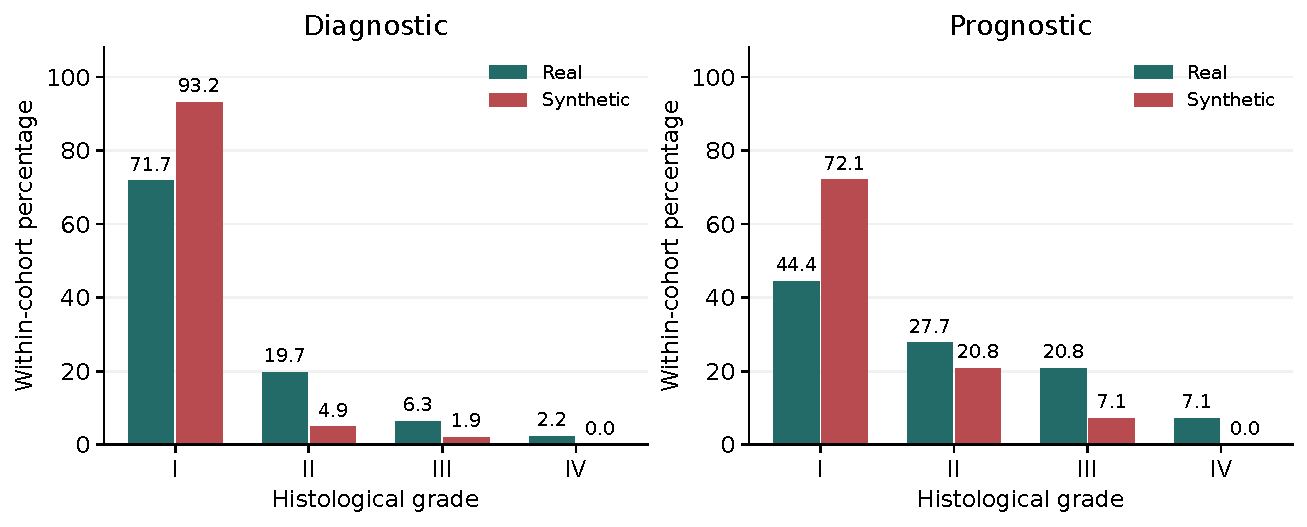
\includegraphics[width=0.92\linewidth]{tabular_transformations/grade_support.pdf}
\caption{Distribution of histological grade in the real and synthetic cohorts.
Bars show the percentage within each cohort. The synthetic bars describe one
generated dataset per task and do not measure variation across repeated
generator fits.}
\label{fig:transforms:grade}
\end{figure}
\FloatBarrier

The consistency checks also compared pairs of variables that describe the same
clinical concept. Nodal stage agreed with its binary indicator in every
synthetic record. Tumour-size fields were less consistent: 46 of 3,000 diagnostic
records and 11 of 462 prognostic records had a size group that did not match their
generated measurement in millimetres. No such disagreement was present in the
real cohorts. Neither synthetic cohort contained duplicate records or an exact
match to a complete real record when the identifier was excluded. The
tumour-size disagreements arose because the continuous measurement and grouped
category were generated separately rather than deriving the group from the
generated millimetre value. The records were retained as produced so that later
analyses describe the generated datasets without post-generation correction.
Section~\ref{sec:similarity-fidelity} examines these and other aspects of
synthetic-data fidelity in greater detail.
\FloatBarrier

\subsection{Appropriate interpretation and transition}
\label{sec:transforms:provenance}

The software versions, random seed and transformation settings were recorded,
but the exact pretrained TabPFN model-weight file was not. The existing datasets
can therefore be analysed exactly as generated, but rerunning the transformations
with a different downloaded weight version may not reproduce identical numerical
values. This is a reproducibility limitation of both transformation routes.

\begin{table}[htbp]
\centering\small
\caption{Appropriate and inappropriate interpretations of the transformed
datasets.}
\label{tab:transforms:use_boundary}
\begin{tabularx}{\linewidth}{@{}p{0.23\linewidth}YY@{}}
\toprule
Dataset & Appropriate use in this study & Interpretation not supported \\
\midrule
Full-cohort embeddings & Exploratory analyses of models using the fixed
TabPFN representation & Strict independent generalisation, survival-specific
representation learning or a clinical meaning for individual coordinates \\
Full-cohort synthetic cohorts & Reproduction of the modelling workflow and
descriptive assessment of similarity, support and internal consistency &
External validation, additional observed patients, a privacy guarantee or an
unbiased test of synthetic augmentation \\
Training-only synthetic cohorts used later & Model augmentation when generation
is restricted to the training patients within each evaluation split & A
replacement for evaluation on untouched real patients or for an independent
external cohort \\
\bottomrule
\end{tabularx}
\end{table}
\FloatBarrier

In summary, the embedding datasets provide new numerical representations of the
original patients, whereas the synthetic datasets provide newly generated
records in the original clinical format. Neither transformation creates new
independent clinical evidence. The following section evaluates diagnostic and
prognostic models using these transformed datasets, with the limitations of
full-cohort construction, approximate censoring representation and incomplete
rare-category support kept explicit.
\FloatBarrier
